\documentclass{article}
\usepackage{pgfplots}
\usepackage{tikz}
\usepgfplotslibrary{fillbetween}
\pgfplotsset{compat=1.18}

\begin{document}

\section*{AWS Braket HHL Circuit Depth Experiment Results}

\noindent
\textbf{Device:} SV1 \\
\textbf{Region:} eu-west-2 \\
\textbf{Matrix Sizes:} $N \in \{2, 4, 8, 16\}$ \\
\textbf{Trials per Size:} 20

\vspace{1em}

\subsection*{1. Circuit Depth Analysis}

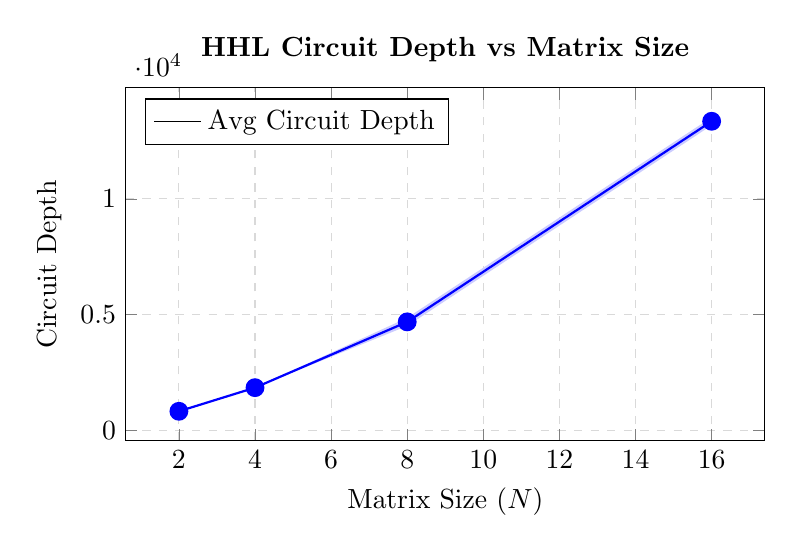
\begin{tikzpicture}
\begin{axis}[
    width=0.8\textwidth,
    height=0.5\textwidth,
    xlabel={Matrix Size ($N$)},
    ylabel={Circuit Depth},
    title={\textbf{HHL Circuit Depth vs Matrix Size}},
    grid=major,
    grid style={dashed, gray!30},
    legend pos=north west,
    mark size=3pt,
]
% Upper bound for error region
\addplot[
    name path=upper,
    draw=none,
] coordinates {
    (2, 817.9) (4, 1839.4) (8, 4858.5) (16, 13527.0)
};

% Lower bound for error region
\addplot[
    name path=lower,
    draw=none,
] coordinates {
    (2, 816.4) (4, 1838.8) (8, 4507.2) (16, 13180.3)
};

% Fill between upper and lower
\addplot[blue!20] fill between[of=upper and lower];

% Main line plot
\addplot[
    blue,
    thick,
    mark=*,
] coordinates {
    (2, 817.1) (4, 1839.1) (8, 4682.9) (16, 13353.6)
};
\addlegendentry{Avg Circuit Depth}

\end{axis}
\end{tikzpicture}

\vspace{0.5em}
\noindent\textbf{Figure 1:} HHL Circuit depth scaling with matrix size. The circuit depth increases significantly as the problem size grows.

\vspace{1em}

\subsection*{2. Total Execution Time}

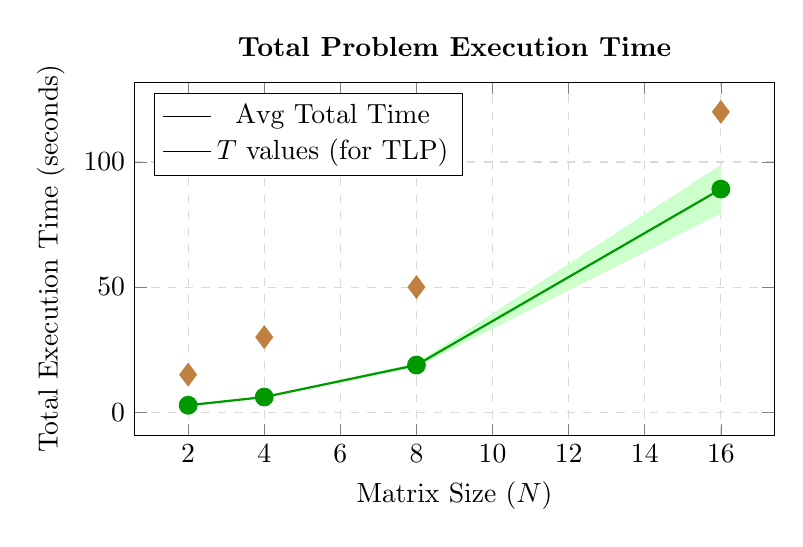
\begin{tikzpicture}
\begin{axis}[
    width=0.8\textwidth,
    height=0.5\textwidth,
    xlabel={Matrix Size ($N$)},
    ylabel={Total Execution Time (seconds)},
    title={\textbf{Total Problem Execution Time}},
    grid=major,
    grid style={dashed, gray!30},
    legend pos=north west,
    mark size=3pt,
]
% Upper bound
\addplot[
    name path=upper,
    draw=none,
] coordinates {
    (2, 3.0375) (4, 6.3391) (8, 19.6287) (16, 98.9039)
};

% Lower bound
\addplot[
    name path=lower,
    draw=none,
] coordinates {
    (2, 2.4996) (4, 5.7629) (8, 18.0359) (16, 79.4126)
};

% Fill between
\addplot[green!20] fill between[of=upper and lower];

% Main time plot
\addplot[
    green!60!black,
    thick,
    mark=*,
] coordinates {
    (2, 2.7685) (4, 6.0510) (8, 18.8323) (16, 89.1582)
};
\addlegendentry{Avg Total Time}

% T values
\addplot[
    brown,
    only marks,
    mark=diamond*,
    mark size=4pt,
] coordinates {
    (2, 15.00) (4, 30.00) (8, 50.00) (16, 120.00)
};
\addlegendentry{$T$ values (for TLP)}

\end{axis}
\end{tikzpicture}

\vspace{0.5em}
\noindent\textbf{Figure 2:} Total problem execution time across different matrix sizes. The diamond markers show the time-lock puzzle $T$ values.

\vspace{1em}

\subsection*{3. Projection Measurement Time}

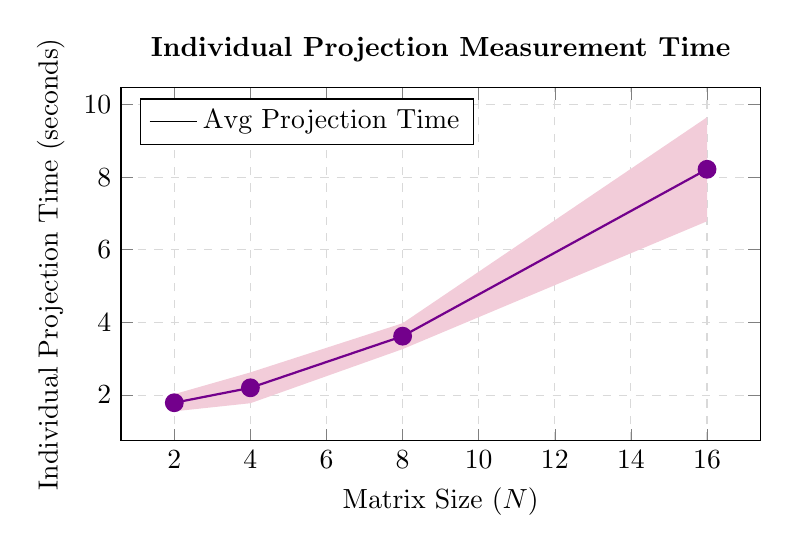
\begin{tikzpicture}
\begin{axis}[
    width=0.8\textwidth,
    height=0.5\textwidth,
    xlabel={Matrix Size ($N$)},
    ylabel={Individual Projection Time (seconds)},
    title={\textbf{Individual Projection Measurement Time}},
    grid=major,
    grid style={dashed, gray!30},
    legend pos=north west,
    mark size=3pt,
]
% Upper bound
\addplot[
    name path=upper,
    draw=none,
] coordinates {
    (2, 2.0251) (4, 2.6245) (8, 3.9781) (16, 9.6466)
};

% Lower bound
\addplot[
    name path=lower,
    draw=none,
] coordinates {
    (2, 1.5524) (4, 1.7755) (8, 3.2653) (16, 6.7842)
};

% Fill between
\addplot[purple!20] fill between[of=upper and lower];

% Projection time plot
\addplot[
    purple!60!blue,
    thick,
    mark=*,
] coordinates {
    (2, 1.7887) (4, 2.2000) (8, 3.6217) (16, 8.2154)
};
\addlegendentry{Avg Projection Time}

\end{axis}
\end{tikzpicture}

\vspace{0.5em}
\noindent\textbf{Figure 3:} Individual projection measurement times for different matrix sizes.

\vspace{1em}

\subsection*{4. Solution Fidelity}

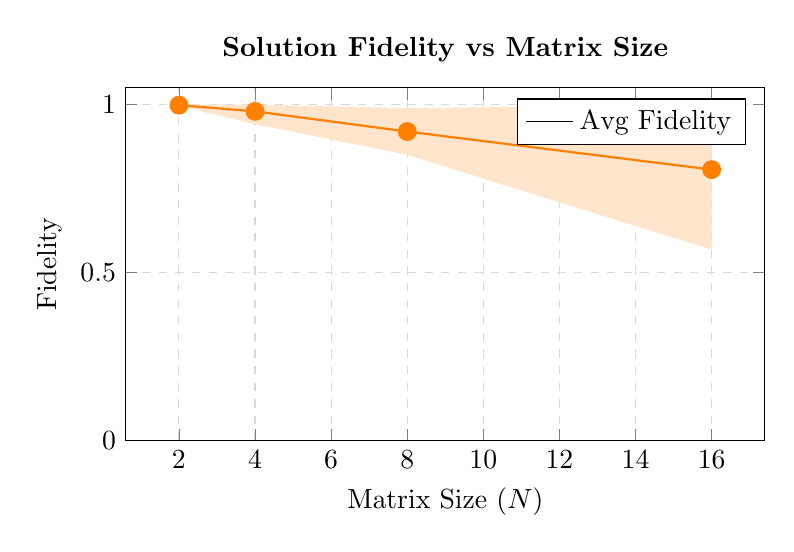
\begin{tikzpicture}
\begin{axis}[
    width=0.8\textwidth,
    height=0.5\textwidth,
    xlabel={Matrix Size ($N$)},
    ylabel={Fidelity},
    title={\textbf{Solution Fidelity vs Matrix Size}},
    grid=major,
    grid style={dashed, gray!30},
    legend pos=north east,
    mark size=3pt,
    ymin=0, ymax=1.05,
]
% Upper bound
\addplot[
    name path=upper,
    draw=none,
] coordinates {
    (2, 1.0000) (4, 1.0000) (8, 0.9895) (16, 1.0000)
};

% Lower bound
\addplot[
    name path=lower,
    draw=none,
] coordinates {
    (2, 0.9962) (4, 0.9420) (8, 0.8506) (16, 0.5683)
};

% Fill between
\addplot[orange!20] fill between[of=upper and lower];

% Fidelity plot
\addplot[
    orange,
    thick,
    mark=*,
] coordinates {
    (2, 0.9985) (4, 0.9801) (8, 0.9200) (16, 0.8068)
};
\addlegendentry{Avg Fidelity}

\end{axis}
\end{tikzpicture}

\vspace{0.5em}
\noindent\textbf{Figure 4:} Solution fidelity across different matrix sizes. Higher fidelity indicates better agreement with the classical solution.

\vspace{1em}

\subsection*{Key Findings Summary}

\begin{itemize}
    \item \textbf{Circuit depth:} 817 to 13354 (16.3$\times$ increase)
    \item \textbf{Fidelity:} 0.807 to 0.999 (avg: 0.926)
    \item \textbf{Execution time:} 2.77s to 89.16s (32.2$\times$ increase)
\end{itemize}

\end{document}
\end{itemize}

\end{document}
